\documentclass[a4paper,12pt]{article}
\usepackage{graphicx}
\usepackage[left=30mm, right=30mm, top=30mm, bottom=35mm]{geometry}
\usepackage{amsmath}
\usepackage{siunitx}
\usepackage{fancyhdr}
\usepackage{url}
\pagestyle{fancy}
%-------------------------------------------------------------------------------
\lhead{\textbf{Spring 2019}}
\rhead{\textbf{CE394M Advanced Analysis in Geotechnical Engineering}}
\cfoot{\thepage}
%-------------------------------------------------------------------------------

\begin{document}
\begin{centering}
	\textbf{
		Assignment 1: Stress equilibrium, compatibility and stiffness matrix\\
		Assigned: 27th January 2019\\
		Due: 8th February 2019\\
	}
\end{centering}

\vspace{1em}
 
\begin{enumerate}
	\item Prove that the following stress-field is a valid lower-bound solution.
	\begin{align*}
		\sigma_{xx} & = c_1 x^3 y - 2c_2 xy + c_3 y\\
		\sigma_{yy} & = c_1 x y^3 - 2c_1 x^3 y\\
		\sigma_{xy} & = -\frac{3}{2}c_1x^2y^2 + c_2 y^2 + \frac{1}{2}c_1 x^4 + c_4
	\end{align*}
	where $c_1$, $c_2$, $c_3$ and $c_4$ are constants.

	\item Determine and describe the stress-state given by the following Airy stress functions:
	\begin{enumerate}
		\item $\phi = Ay^2$ 
		\item $\phi = Bxy$
	\end{enumerate}
	Are these stresses valid for an isotropic elastic element? Note: please refer \url{https://en.wikiversity.org/wiki/Airy_stress_function} on how to determine cauchy stress components from an Airy function.

	\item Determine whether the following strain fields are possible in a two-dimensional continous body:
	
	\begin{enumerate}
		\item $\!
			\begin{aligned}[t]
				\varepsilon = %			
				\begin{bmatrix}
				\varepsilon_{xx} & \varepsilon_{xy} \\
				\varepsilon_{xy} & \varepsilon_{yy} \\
				\end{bmatrix} = 
				\begin{bmatrix}
				c_1(x^2 + y^2) & c_1 xy \\
				c_1 xy & c_2 y^2 \\
				\end{bmatrix}
			\end{aligned}$
		\item $\!
			\begin{aligned}[t]
				\varepsilon = %			
				\begin{bmatrix}
					\varepsilon_{xx} & \varepsilon_{xy} \\
					\varepsilon_{xy} & \varepsilon_{yy} \\
				\end{bmatrix} = 
				\begin{bmatrix}
				c_1(x^2 + y^3) & 3c_1 xy^2/2 \\
				3c_1 xy^2/2 & c_2 x^3 \\
				\end{bmatrix}
			\end{aligned}$		
	\end{enumerate}
	
	\item Given the one-dimensional steel bar below, which is represented by two elements, 
	determine the system's global stiffness matrix ($\mathbf{K}$).  The bar has a cross sectional area 
	($A$) of~\SI{5E-04}{\meter\square} and Young’s modulus ($E$) of \SI{20}{\giga\pascal}. Please note that the deformation of an elastic bar is governed as follows:  $\delta = FL/AE$, where $F$ is the 
	applied force leading to a displacement of $\delta$.  Also, note that this bar can be characterized in one dimension only with just two degrees of freedom (i.e. displacement at each of the two nodes in the $x$ direction only).
	
	\begin{figure}[!h]
		\centering
		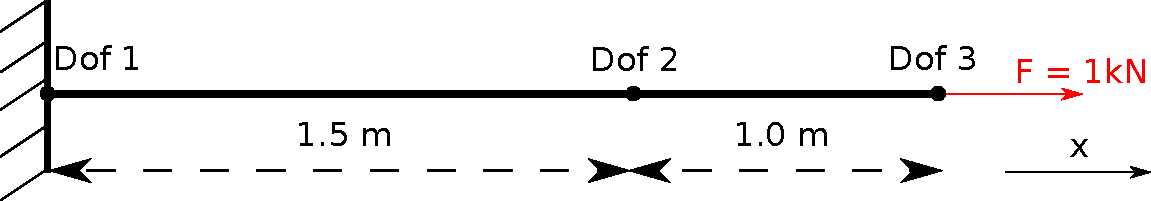
\includegraphics[width=0.75\textwidth]{figs/cantilever.pdf}
	\end{figure}
	
	Assuming a horizontal force $F_x = $\SI{1}{\kilo\newton} at DOF 3, solve for displacements at all degrees of freedom. You are encouraged to use Jupyter notebooks to solve the linear system of equations.
\end{enumerate}

\end{document}

